\documentclass[aspectratio=169]{beamer}
\usetheme{metropolis}

\beamertemplatenavigationsymbolsempty
\setbeamertemplate{footline}[frame number]

% Encoding
\usepackage{ae,lmodern}
\usepackage[utf8]{inputenc}
\usepackage[T1]{fontenc}

% Language
\usepackage[main=french,english]{babel}

\usepackage{url}
\usepackage{tabularx}
\usepackage{booktabs}
\usepackage{listings}
\usepackage{hyperref}
\usepackage{qrcode}
\usepackage{graphicx}
\usepackage{multicol}
\usepackage{svg}
\svgsetup{inkscapelatex=false}

\lstset{
    numbers=none,
    stepnumber=1,
    numbersep=5pt,
    basicstyle=\ttfamily\scriptsize,
    keywordstyle=\color{keyword}\bfseries\ttfamily,
    commentstyle=\color{comment}\ttfamily,
    stringstyle=\color{string}\ttfamily,
    identifierstyle=,
    showstringspaces=false,
    columns=flexible,
    keepspaces=true,
    breaklines=true,
    captionpos=b,
    tabsize=2,
    frame=none,
}

\definecolor{keyword}{HTML}{2771a3}
\definecolor{pattern}{HTML}{b53c2f}
\definecolor{string}{HTML}{be681c}
\definecolor{relation}{HTML}{7e4894}
\definecolor{variable}{HTML}{107762}
\definecolor{comment}{HTML}{8d9094}

\lstdefinelanguage{cypher}
{
    morekeywords={MATCH, OPTIONAL, WHERE, NOT, AND, OR, XOR, RETURN, DISTINCT, ORDER, BY, ASC, ASCENDING, DESC, DESCENDING, UNWIND, AS, UNION, WITH, ALL, CREATE, DELETE, DETACH, REMOVE, SET, MERGE, SET, SKIP, LIMIT, IN, CASE, WHEN, THEN, ELSE, END, INDEX, DROP, UNIQUE, CONSTRAINT, EXPLAIN, PROFILE, START, CALL},
    morecomment=[l]{//},
}

\lstdefinelanguage{http}{%
    morekeywords=[1]{HTTP,%
    GET,POST,PUT,HEAD,DELETE,PATCH,OPTIONS,CONNECT,TRACE,%
    OK,Precondition,Failed,Not,Modified,Acceptable,%
    Created,Found,Accepted,No,Content,Gone,Multiple,Choices,See,Other,Method,Allowed,%
    Unsupported,Media,Type,Required%
    },%
    morekeywords=[2]{%
        Accept,Accept-Encoding,Accept-Language,Alternates,%
        Content-Type,Content-Language,Content-Encoding,Content-Location,Content-Length,%
        If-Match,If-None-Match,If-Modified-Since,If-Unmodified-Since,%
        ETag,Last-Modified,Negotiate,TCN,Vary,%
        Cache-control,%
        Allow,%
        Date,%
        Host,%
        Location,%
        Server,%
        User-Agent,%
    },%
    alsodigit=-,%
    morestring=[b]",%
    morecomment=[l]\$,%
    morecomment=[s]{[}{]},%
}[keywords,comments,strings]

\hyphenation{onepoint}
\newcommand{\etal}{\textit{et al}. }
\newcommand{\ie}{\textit{i}.\textit{e}. }
\newcommand{\eg}{\textit{e}.\textit{g}. }

\begin{document}
    \title{Introduction au génie logiciel}

\author{Sébastien Bertrand}

\institute{
    
\includegraphics[scale=1, height=0.6cm]{figures/header/logo-ensc}
    
\includegraphics[scale=1, height=0.6cm]{figures/header/logo-onepoint}
}

\date{\today}

\frame[plain,noframenumbering]{\titlepage}

    % Présentation générale, technologie front back autres, objectif tp
% README, markdown, HTTP, Console
% Rappel POO ? Structure etc
% https://en.wikipedia.org/wiki/Software_design#Design_considerations
\section{Introduction}
\label{sec:introduction}

\begin{frame} \frametitle{Titre} \end{frame}
\begin{frame} \frametitle{Titre} \end{frame}
\begin{frame} \frametitle{Titre} \end{frame}
\begin{frame} \frametitle{Titre} \end{frame}
\begin{frame} \frametitle{Titre} \end{frame}
\begin{frame} \frametitle{Titre} \end{frame}
\begin{frame} \frametitle{Titre} \end{frame}
\begin{frame} \frametitle{Titre} \end{frame}
\begin{frame} \frametitle{Titre} \end{frame}
\begin{frame} \frametitle{Titre} \end{frame}
\begin{frame} \frametitle{Titre} \end{frame}
\begin{frame} \frametitle{Titre} \end{frame}
\begin{frame} \frametitle{Titre} \end{frame}
\begin{frame} \frametitle{Titre} \end{frame}
\begin{frame} \frametitle{Titre} \end{frame}
\begin{frame} \frametitle{Titre} \end{frame}
\begin{frame} \frametitle{Titre} \end{frame}
\begin{frame} \frametitle{Titre} \end{frame}
\begin{frame} \frametitle{Titre} \end{frame}
\begin{frame} \frametitle{Titre} \end{frame}
\begin{frame} \frametitle{Titre} \end{frame}
\begin{frame} \frametitle{Titre} \end{frame}
\begin{frame} \frametitle{Titre} \end{frame}
\begin{frame} \frametitle{Titre} \end{frame}
\begin{frame} \frametitle{Titre} \end{frame}
\begin{frame} \frametitle{Titre} \end{frame}
\begin{frame} \frametitle{Titre} \end{frame}
\begin{frame} \frametitle{Titre} \end{frame}
\begin{frame} \frametitle{Titre} \end{frame}
\begin{frame} \frametitle{Titre} \end{frame}

    \section{Modélisation UML}
\label{sec:uml}

% todo: Avant le cours relire les chapitres 3, 4, 5 et 11.

\begin{frame}
    \frametitle{Définition}
    \begin{columns}
        \begin{column}{0.5\textwidth}
            Le langage de modélisation unifié (UML) est une famille de \textbf{notations graphiques},
            soutenues par un méta-modèle unique,
            qui aident \underline{à décrire et à concevoir} des systèmes logiciels,
            en particulier des systèmes logiciels construits à l'aide du style orienté objet.
        \end{column}
        \begin{column}{0.5\textwidth}
            \centering
            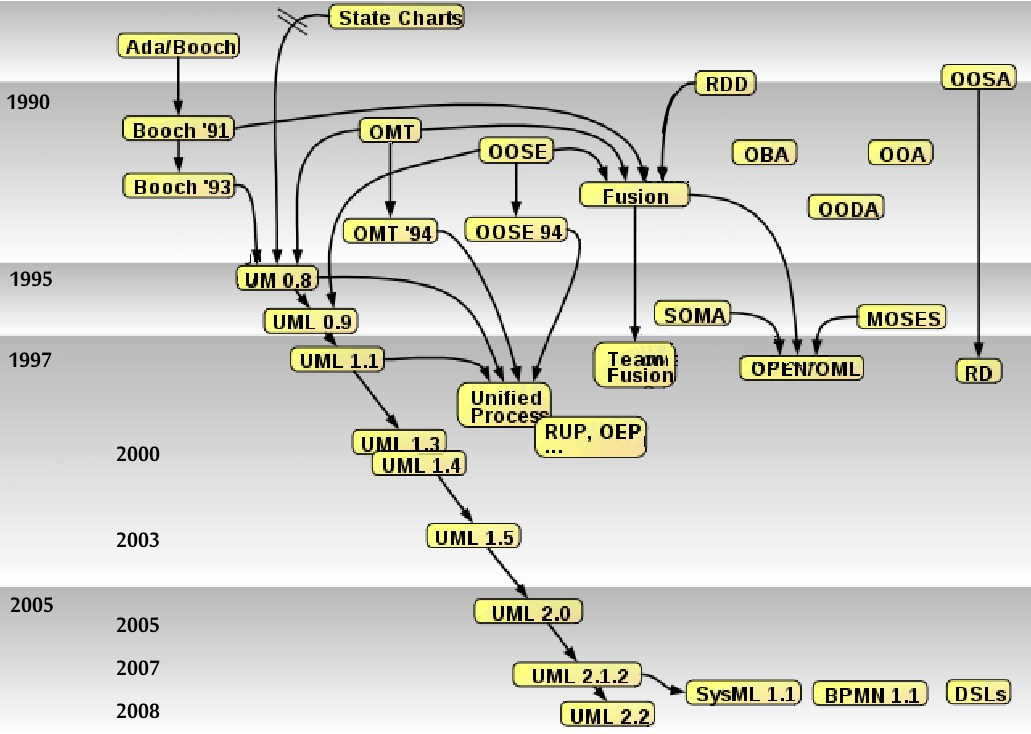
\includegraphics[width=\linewidth]{figures/uml/uml-historie}
        \end{column}
    \end{columns}
\end{frame}

\begin{frame}
    \frametitle{Les diagrammes}
    \begin{itemize}
        \item Diagrammes de structure
        \item Diagrammes de comportement
    \end{itemize}
    \centering
    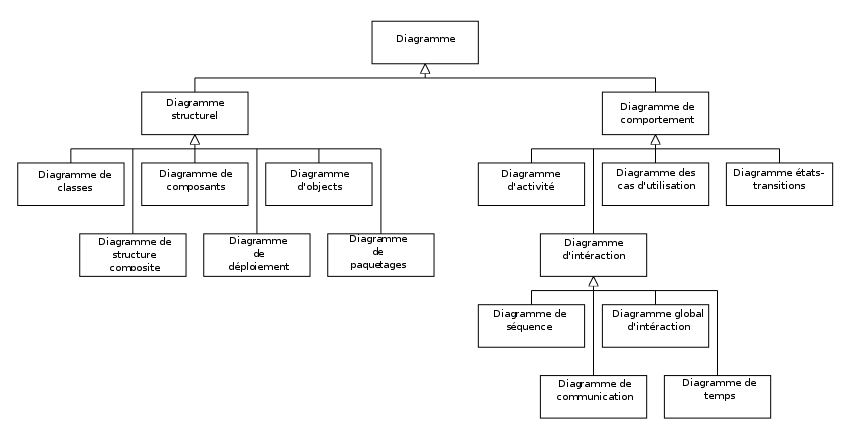
\includegraphics[height=0.4\linewidth]{figures/uml/uml-diagrammes}
\end{frame}

\subsection{Diagramme de classes}
\label{subsec:diagramme-classes}

\begin{frame}
    \frametitle{Diagramme de classes}
    Un diagramme de classes \textbf{décrit les types d'objets du système}
    et les différents types de \underline{relations statiques} qui existent entre eux.
    Les diagrammes de classes montrent également
    \emph{les propriétés et les opérations} d'une classe
    ainsi que les contraintes qui s'appliquent à la manière dont les objets sont connectés.
\end{frame}

\begin{frame}
    \frametitle{Une classe}
    \centering
    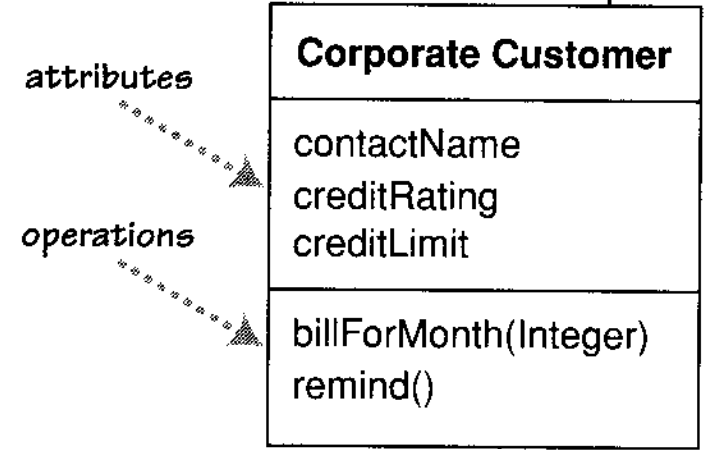
\includegraphics[height=0.5\linewidth]{figures/uml/classe}
\end{frame}

\begin{frame}
    \frametitle{La généralisation (héritage)}
    \centering
    \includegraphics[height=0.5\linewidth]{figures/uml/classe-héritage}
\end{frame}

\begin{frame}
    \frametitle{Un diagramme de classes simple}
    \centering
    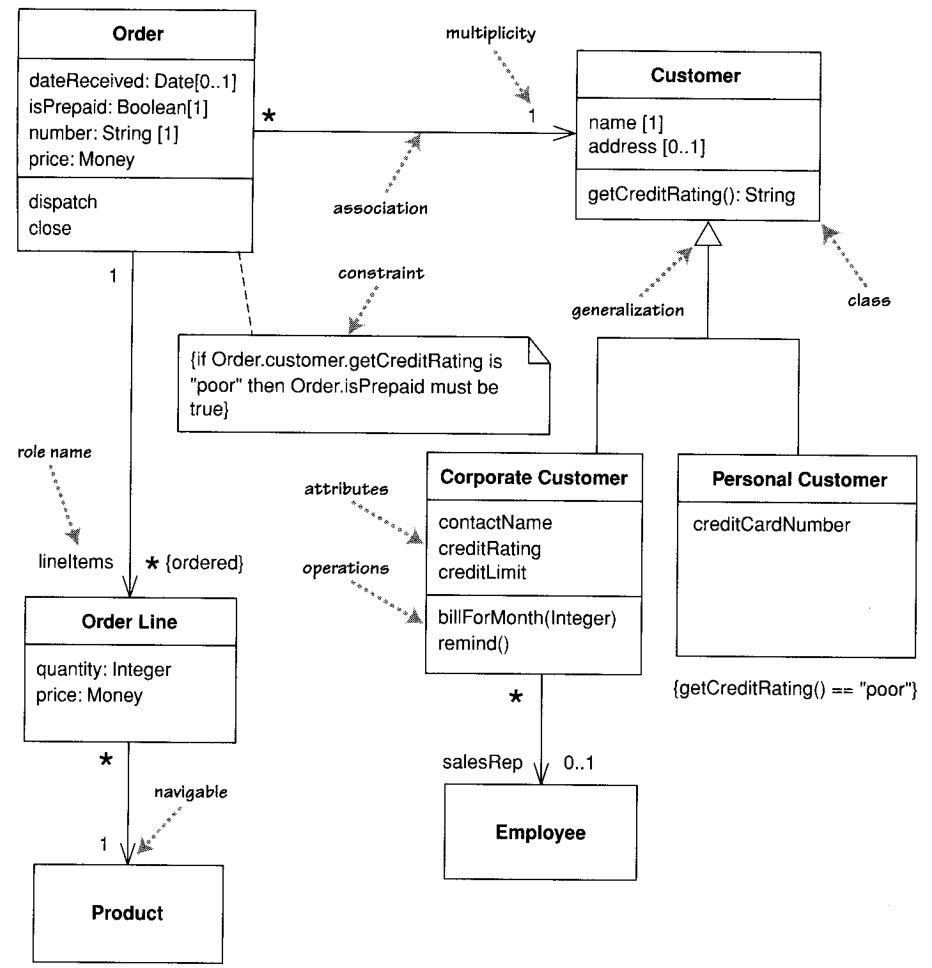
\includegraphics[height=0.5\linewidth]{figures/uml/classe-complet}
\end{frame}

\begin{frame}
    \frametitle{Les propriété comme association ou attribut ?}
    \centering
    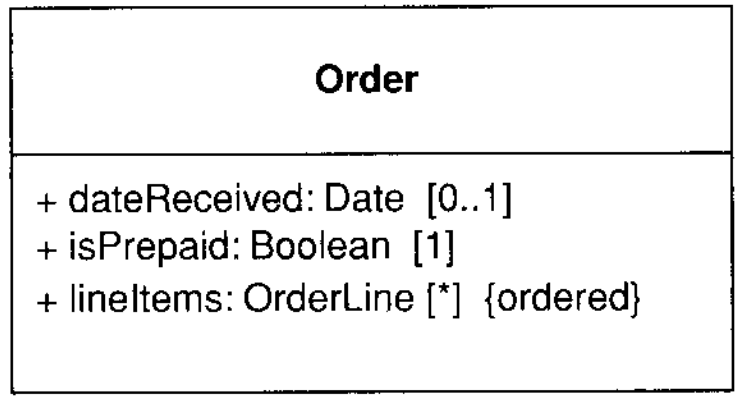
\includegraphics[height=0.15\linewidth]{figures/uml/classe-propriétés-1}
    \vfill
    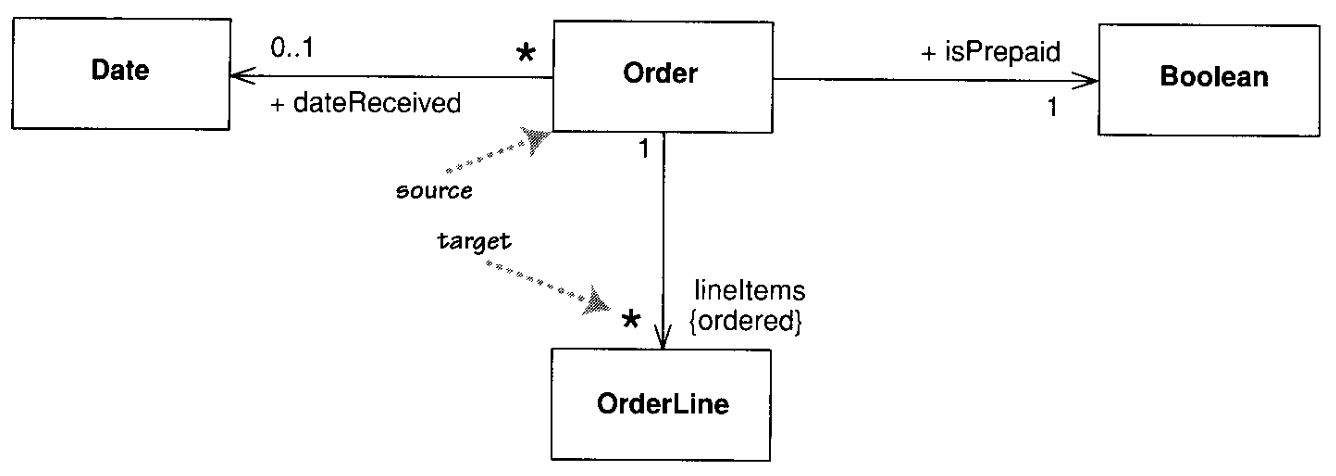
\includegraphics[height=0.25\linewidth]{figures/uml/classe-propriétés-2}
\end{frame}

\begin{frame}
    \frametitle{Cardinalité et directionnalité}
    \begin{itemize}
        \item \textbf{Optionnel} implique une limite inférieure de 0 ;
        \item \textbf{Obligatoire} implique une limite inférieure de 1 ou éventuellement plus ;
        \item \textbf{Une valeur unique} implique une limite supérieure de 1 ;
        \item \textbf{Une valeur multiple} implique une limite supérieure à 1 (généralement *).
    \end{itemize}
    \vfill
    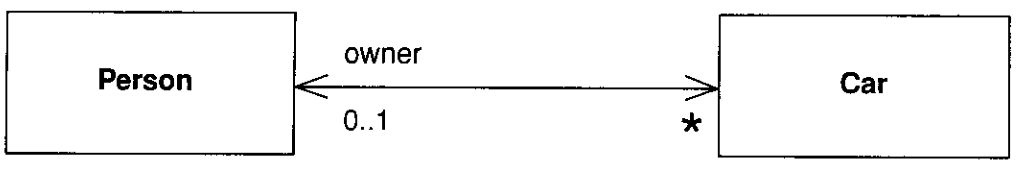
\includegraphics[width=\textwidth]{figures/uml/classe-bidirectionnelle}
\end{frame}

\begin{frame}
    \frametitle{Dépendance}
    Une dépendance existe entre deux éléments si des
    modifications de la définition d'un élément (le fournisseur)
    peuvent entraîner des modifications de l'autre (le client).
    \vfill
    \includegraphics[width=\textwidth]{figures/uml/classe-dépendance}
\end{frame}

\begin{frame}
    \frametitle{Agrégation et composition}
    \centering
    \includegraphics[width=\textwidth]{figures/uml/classe-agrégation-composition}
\end{frame}

\begin{frame}
    \frametitle{Implémentation}
    \centering
    \includegraphics[height=0.5\linewidth]{figures/uml/classe-implémentation}
\end{frame}

\begin{frame}
    \frametitle{Diagrammme de classes PlantUML}
    \begin{columns}
        \begin{column}{0.4\textwidth}
            \lstinputlisting[
                basicstyle=\tiny,
                label=lst:classe-plantuml]
            {figures/uml/classe-plantuml.puml}
        \end{column}
        \begin{column}{0.6\textwidth}
            \centering
            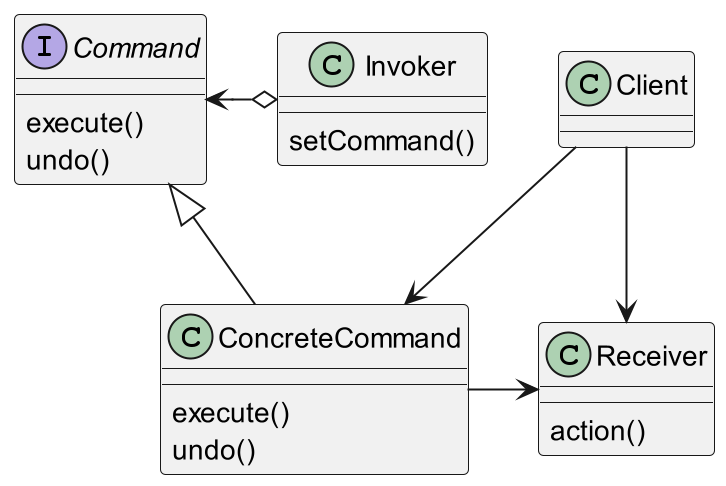
\includegraphics[width=0.8\linewidth]{figures/uml/classe-plantuml}
        \end{column}
    \end{columns}
\end{frame}

\subsection{Diagramme de séquence}
\label{subsec:diagramme-sequence}

\begin{frame}
    \frametitle{Diagramme de séquence}
    Un diagramme de séquence montre la \textbf{collaboration dynamique} entre plusieurs objets
    en décrivant \emph{l’ordre temporel} dans lequel les messages sont envoyés entre eux.
\end{frame}

\begin{frame}
    \frametitle{Un permier diagramme de séquence}
    \centering
    \includegraphics[height=0.5\linewidth]{figures/uml/sequence-exemple-centralisé}
\end{frame}

\begin{frame}
    \frametitle{Le même, mais distribué au lieu de centralisé}
    \centering
    \includegraphics[height=0.5\linewidth]{figures/uml/sequence-exemple-distribué}
\end{frame}

\begin{frame}
    \frametitle{Création et suppression des participants}
    \centering
    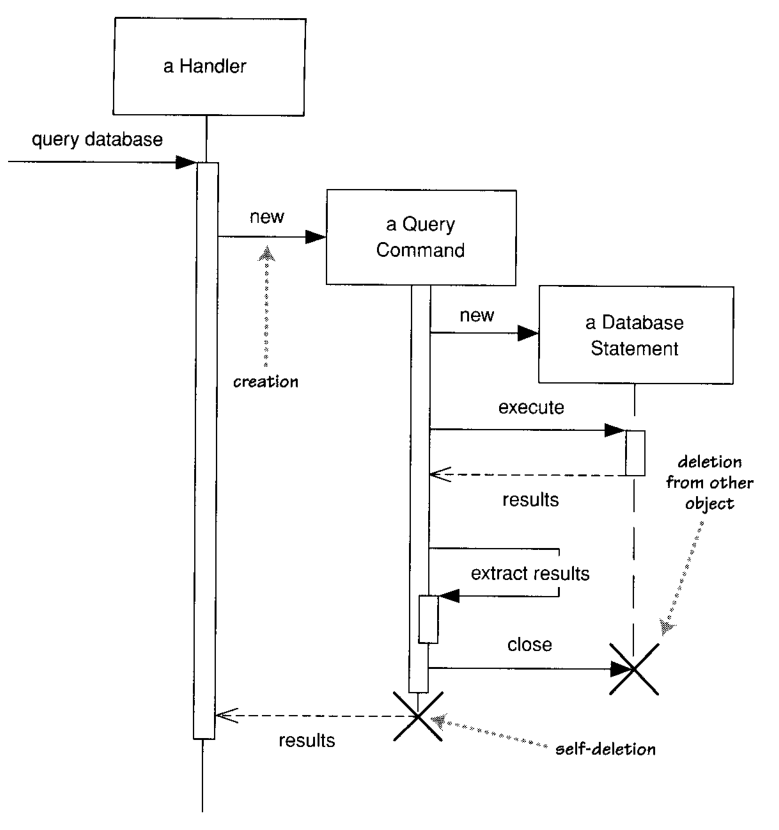
\includegraphics[height=0.5\linewidth]{figures/uml/sequence-creation-deletion}
\end{frame}

\begin{frame}
    \frametitle{Fragments : Boucles, conditions, etc}
    \centering
    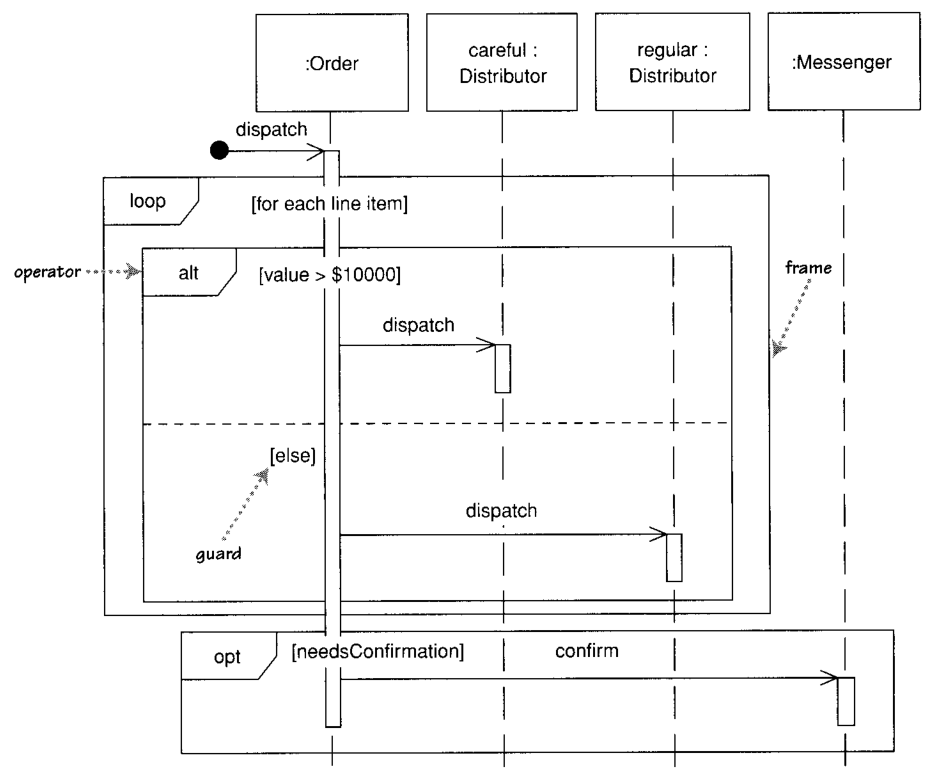
\includegraphics[height=0.5\linewidth]{figures/uml/sequence-fragments}
\end{frame}

\begin{frame}
    \frametitle{Quelques opérateurs de fragments}
    \begin{itemize}
        \item \textbf{alt} : Fragments multiples alternatifs, seulement celui dont la garde est vraie s'exécutera.
        \item \textbf{opt} : Facultatif, le fragment ne s'exécute que si la condition fournie est vrai.
        \item \textbf{par} : Parallèle, chaque fragment est traité en parallèle.
        \item \textbf{loop} : Boucle, le fragment peut s'exécuter plusieurs fois et la garde indique la base de l'itération.
        \item \textbf{ref} : Référence, fait référence à une interaction définie sur un autre diagramme.
    \end{itemize}
\end{frame}

\begin{frame}
    \frametitle{Diagramme de séquence PlantUML}
    \begin{columns}
        \begin{column}{0.4\textwidth}
            %todo: problème d'affichage du listing...
            \lstinputlisting[
                basicstyle=\tiny,
                label=lst:sequence-plantuml]
            {figures/uml/sequence-plantuml.puml}
        \end{column}
        \begin{column}{0.6\textwidth}
            \centering
            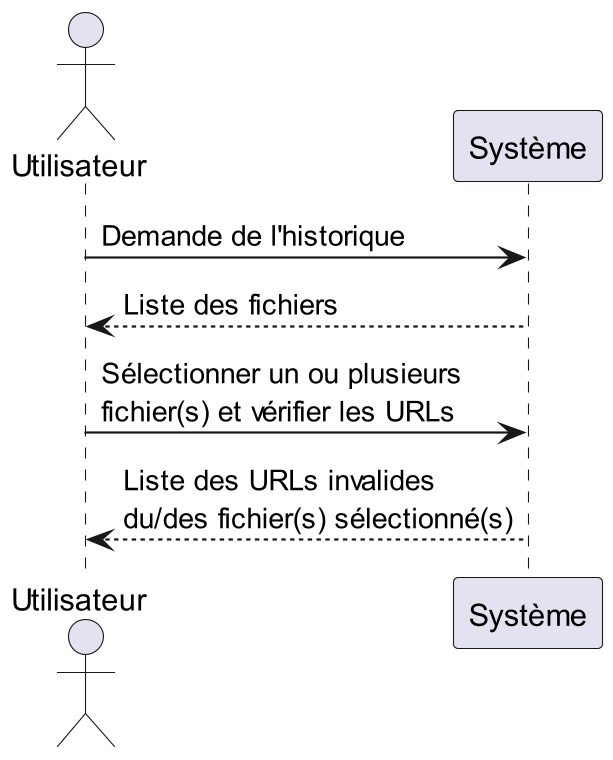
\includegraphics[height=0.8\linewidth]{figures/uml/sequence-plantuml}
        \end{column}
    \end{columns}
\end{frame}

\subsection{Diagramme d'activité}
\label{subsec:diagramme-activite}

\begin{frame}
    \frametitle{Diagramme d'activité}
    Les diagrammes d'activités sont une technique pour décrire
    la \textbf{logique procédurale}, les \textbf{processus métier} et les \textbf{flux de travail}.
\end{frame}

\begin{frame}
    \frametitle{Un exemple simple de diagramme d'activité}
    \centering
    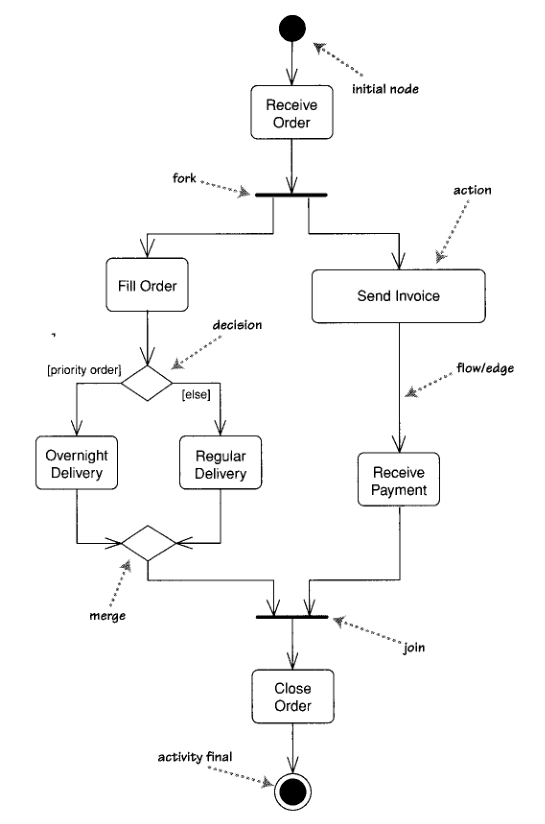
\includegraphics[height=0.5\linewidth]{figures/uml/activite-exemple}
\end{frame}

\begin{frame}
    \frametitle{Diagramme d'activité PlantUML}
    \begin{columns}
        \begin{column}{0.4\textwidth}
            %todo: problème d'affichage du listing...
            \lstinputlisting[
                basicstyle=\tiny,
                label=lst:activite-plantuml]
            {figures/uml/activite-plantuml.puml}
        \end{column}
        \begin{column}{0.6\textwidth}
            \centering
            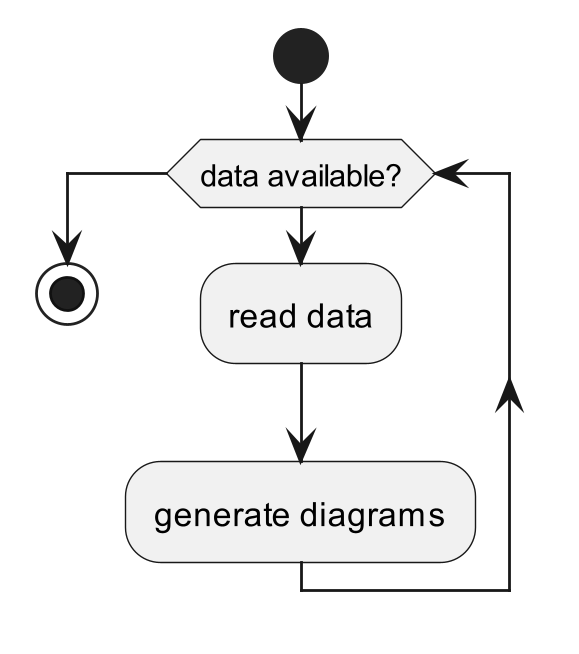
\includegraphics[height=0.8\linewidth]{figures/uml/activite-plantuml}
        \end{column}
    \end{columns}
\end{frame}

\begin{frame}
    \frametitle{Un livres de référence}
    \centering
    
\includegraphics[height=0.5\linewidth]{figures/uml/uml-book}
\end{frame}

    \section{L'environnement du développeur}
\label{sec:environnement}

\subsection{L'environnement}
\label{subsec:environnement}

\begin{frame}
    \frametitle{Environnement de développement intégré (IDE)}

    Un environnement de développement intégré est une application logicielle
    qui fournit des \emph{fonctionnalités complètes pour le développement de logiciels}.

    Les IDE sont conçus pour \textbf{maximiser la productivité des programmeurs}
    en fournissant des composants étroitement intégrés qui fournissent de nombreuses fonctionnalités :
    \begin{itemize}
        \item Edition de texte ;
        \item Vérification de syntaxe ;
        \item Gestion de version ;
        \item Compilation ;
        \item Gestion des tests ;
        \item Débogage de logiciel ;
        \item \ldots
    \end{itemize}
\end{frame}

\begin{frame}
    \frametitle{Une usine à gaz\ldots}
    \centering
    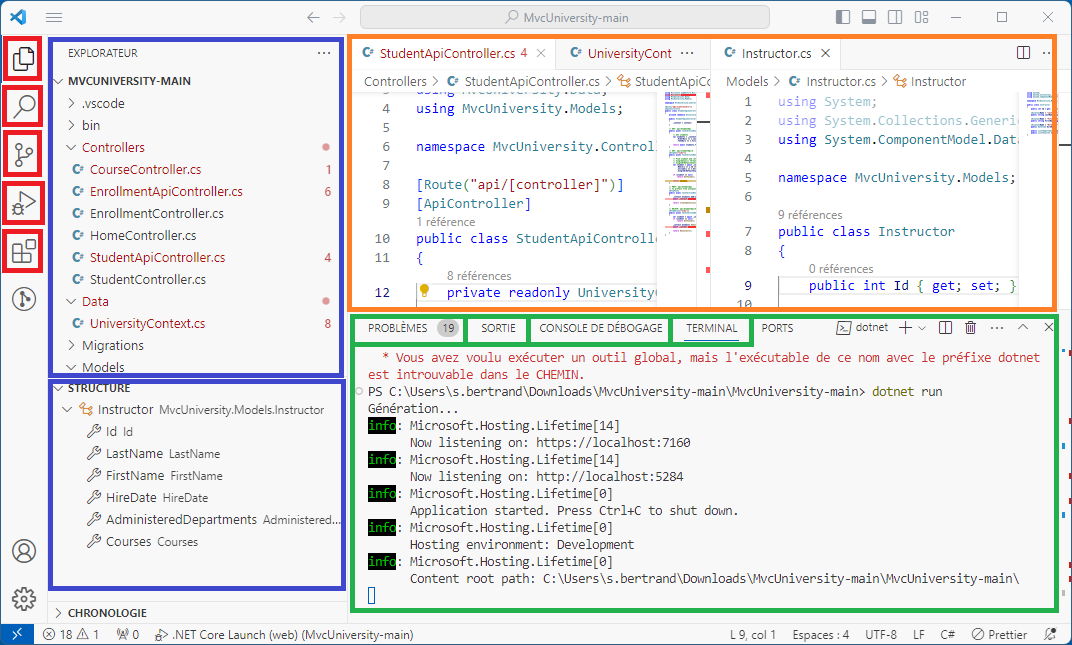
\includegraphics[height=0.5\linewidth]{figures/environnement/vscode}
\end{frame}

\begin{frame}
    \frametitle{Définition et références}
    \centering
    \Huge
    \textbf{CTRL + CLIC}

    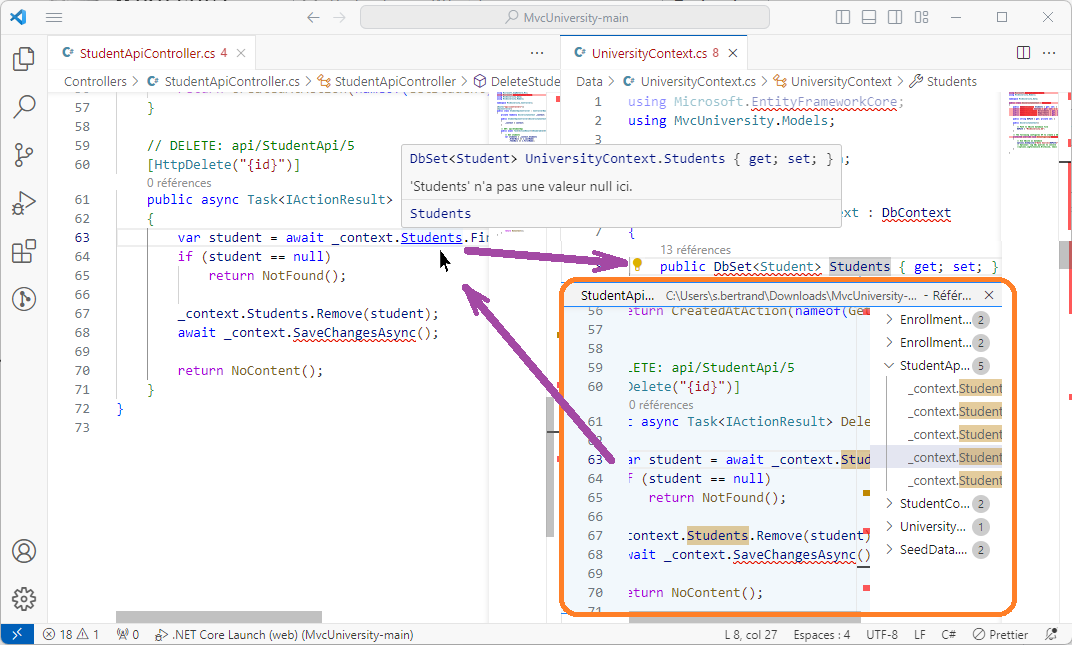
\includegraphics[height=0.4\linewidth]{figures/environnement/controle-clic}
\end{frame}

\begin{frame}
    \frametitle{Recherche}
    \centering
    \Huge
    \textbf{CTRL + (MAJ) + F}

    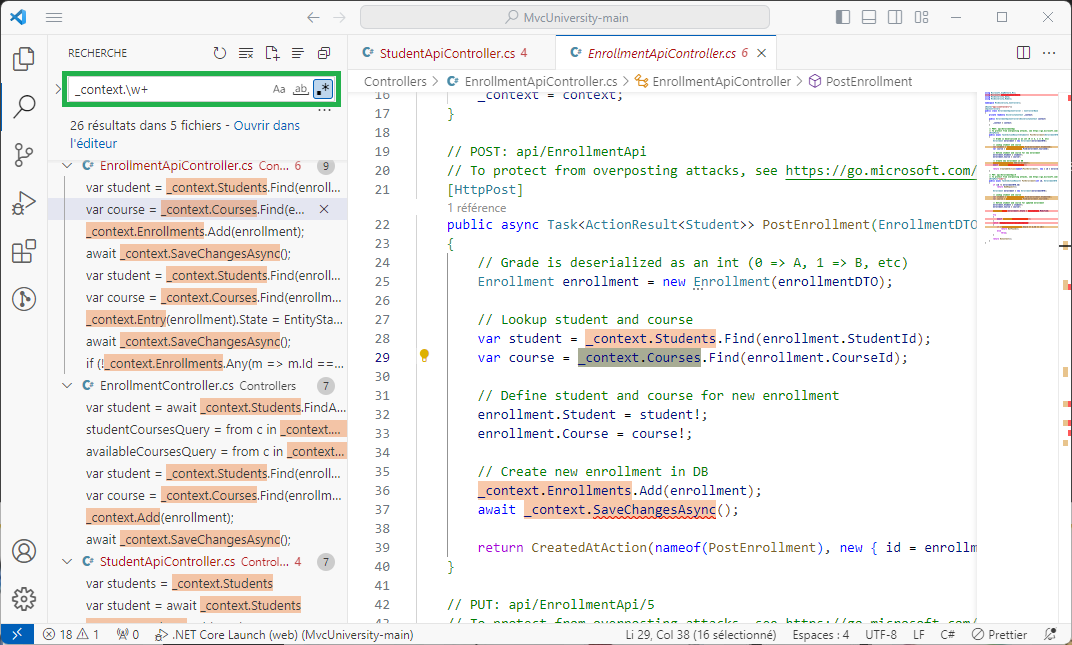
\includegraphics[height=0.4\linewidth]{figures/environnement/rechercher}
\end{frame}

\begin{frame}[fragile]
    \frametitle{Les expressions régulières}
    \begin{columns}
        \begin{column}{0.7\textwidth}
            \begin{itemize}
                \item \verb|[A-Z]\w+| : n'importe quel mot qui commence par une majuscule ;
                \item \verb|.*| : n'importe quelle suite de caractère (sauf \verb|\n| et \verb|\r|) ;
                \item \verb|a*\w+| : \verb|a*| ne sert à rien ;
                \item \verb|[+-]?(\d*[.])?\d+| : Nombre à virgule flottante.
            \end{itemize}
        \end{column}
        \begin{column}{0.3\textwidth}
            \centering

            \qrcode[height=70pt]{https://regexr.com/}
        \end{column}
    \end{columns}
\end{frame}

\begin{frame}
    \frametitle{Remplacer à l'aide des expressions régulières}
    \centering
    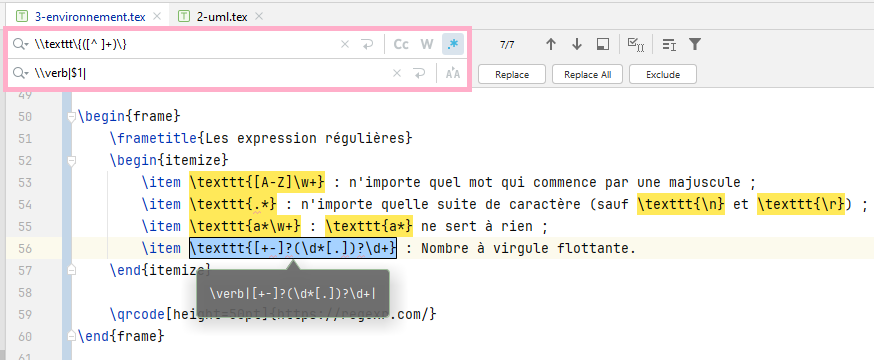
\includegraphics[height=0.4\linewidth]{figures/environnement/remplacer}
\end{frame}

\begin{frame}
    \frametitle{Renommer un élément de programme}
    \centering
    \Huge
    \textbf{F2}

    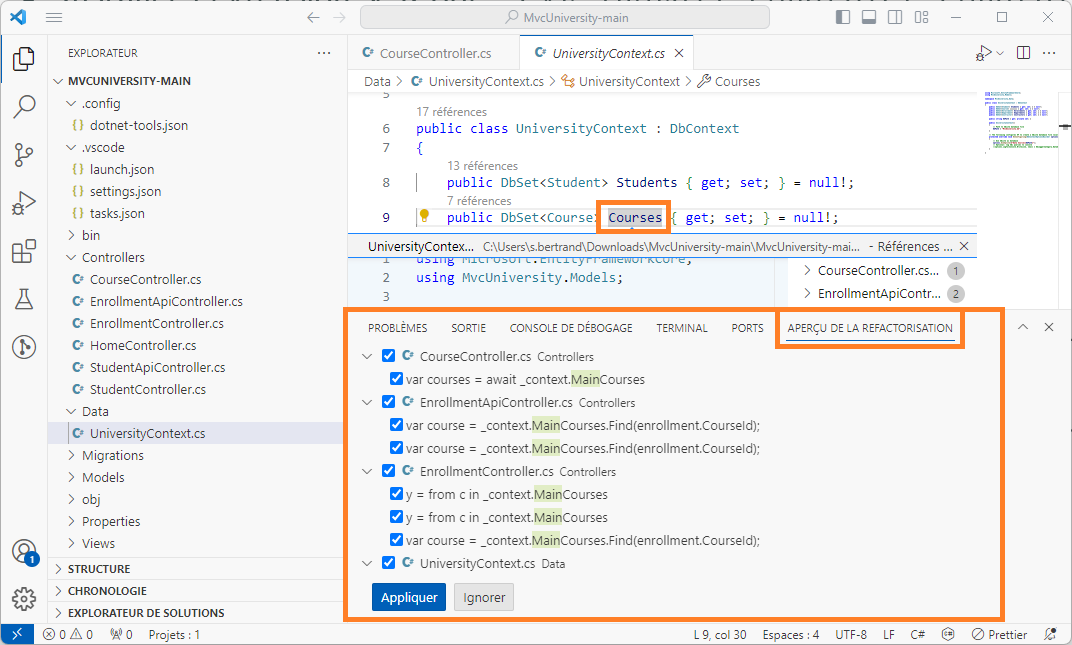
\includegraphics[height=0.4\linewidth]{figures/environnement/renommer}
\end{frame}

\begin{frame}
    \frametitle{Refactoriser}
    \centering
    \Huge\textbf{CTRL + MAJ + R}\\
    \normalsize Installer l'extension VSCode : \texttt{ext install ms-dotnettools.csdevkit} (CTRL+P)

    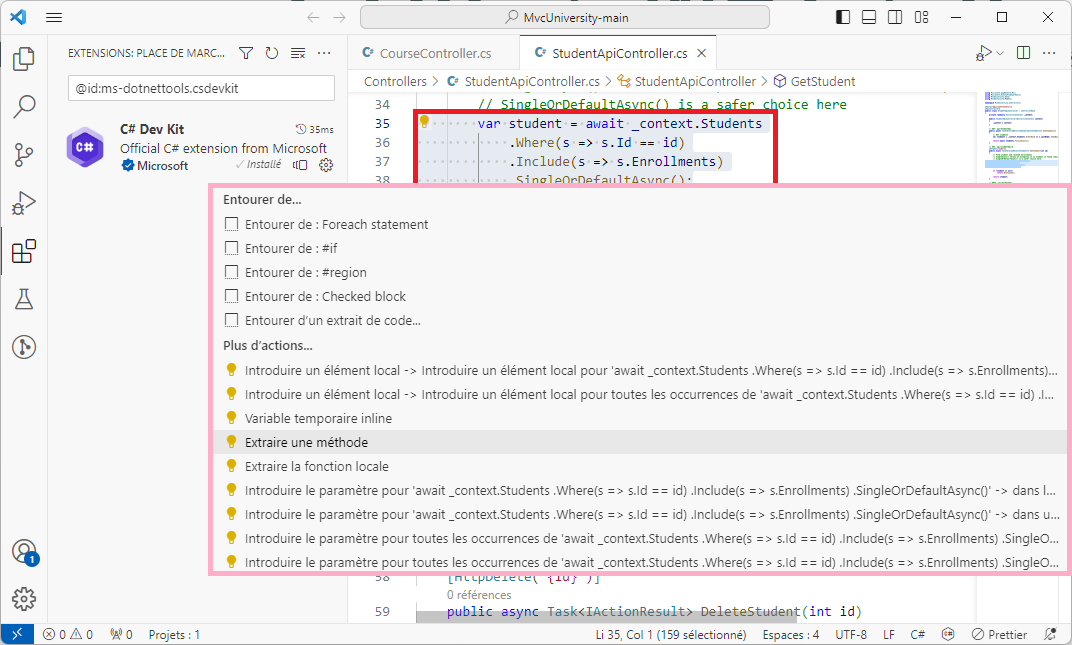
\includegraphics[height=0.35\linewidth]{figures/environnement/refactoriser}
\end{frame}

\begin{frame}
    \frametitle{Editer plusieurs ligne à la fois}
    \centering
    \Huge\textbf{ALT + CLIC}

    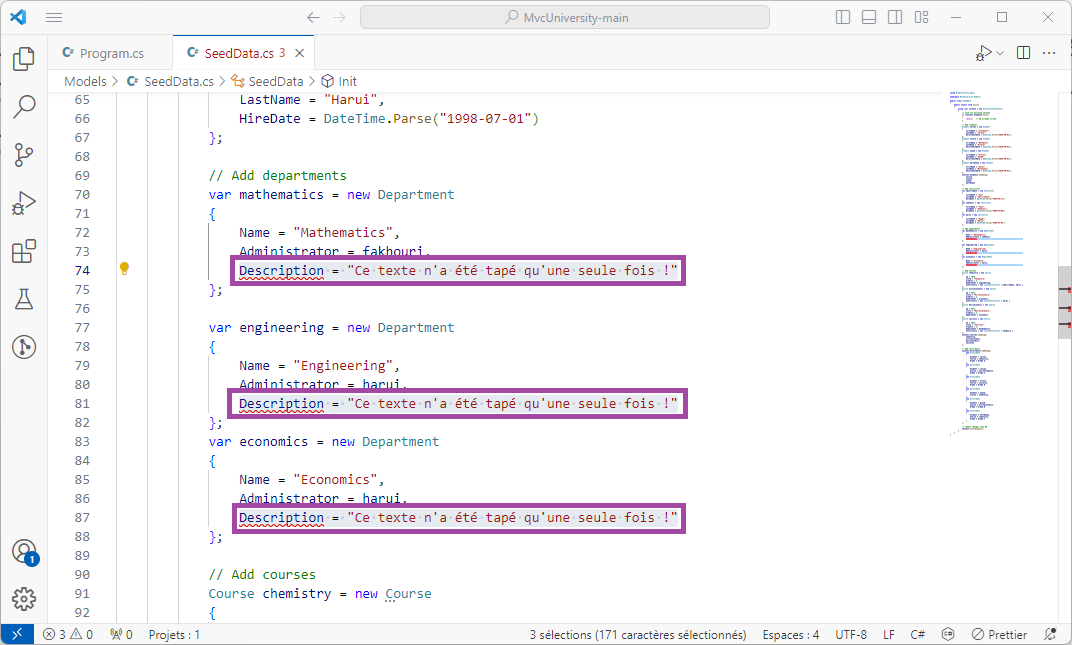
\includegraphics[height=0.4\linewidth]{figures/environnement/multi-edition}
\end{frame}

\begin{frame}
    \frametitle{Présenter le code source}
    \centering
    \Huge
    \textbf{CTRL + ALT + F}

    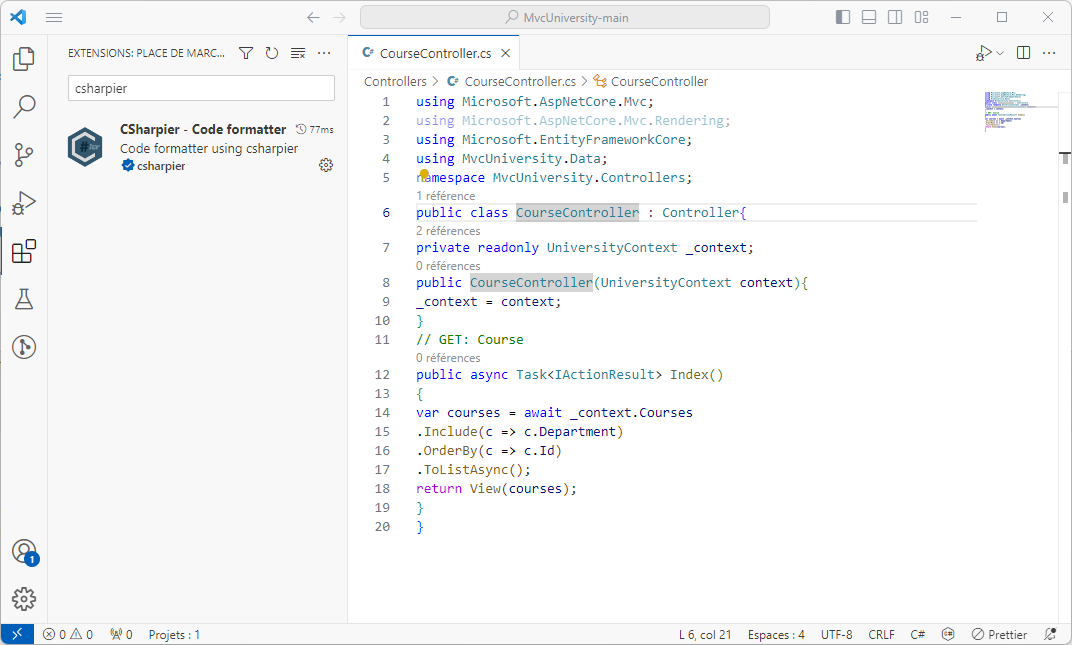
\includegraphics[height=0.4\linewidth]{figures/environnement/mise-en-forme}
\end{frame}

\begin{frame}[fragile]
    \frametitle{Installer CSharpier}
    \centering
    \begin{itemize}
        \item Installer l'outil DotNet : \texttt{dotnet tool install csharpier -g}
        \item Installer l'extension VSCode : \texttt{ext install csharpier.csharpier-vscode} (CTRL+P)
        \item Configurer en tant que formateur par défaut (Paramètres)
        \item Activer \enquote{Format On Save}
        \item Editer le fichier \texttt{/.vscode/settings.json}):
    \end{itemize}

    \begin{verbatim}
    "editor.defaultFormatter": "csharpier.csharpier-vscode",
    "[csharp]": {
        "editor.defaultFormatter": "csharpier.csharpier-vscode"
    },
    \end{verbatim}
\end{frame}

\begin{frame}
    \frametitle{Une commande pour les gouverner toutes}
    \centering
    \Huge
    \textbf{CTRL + MAJ + P}

    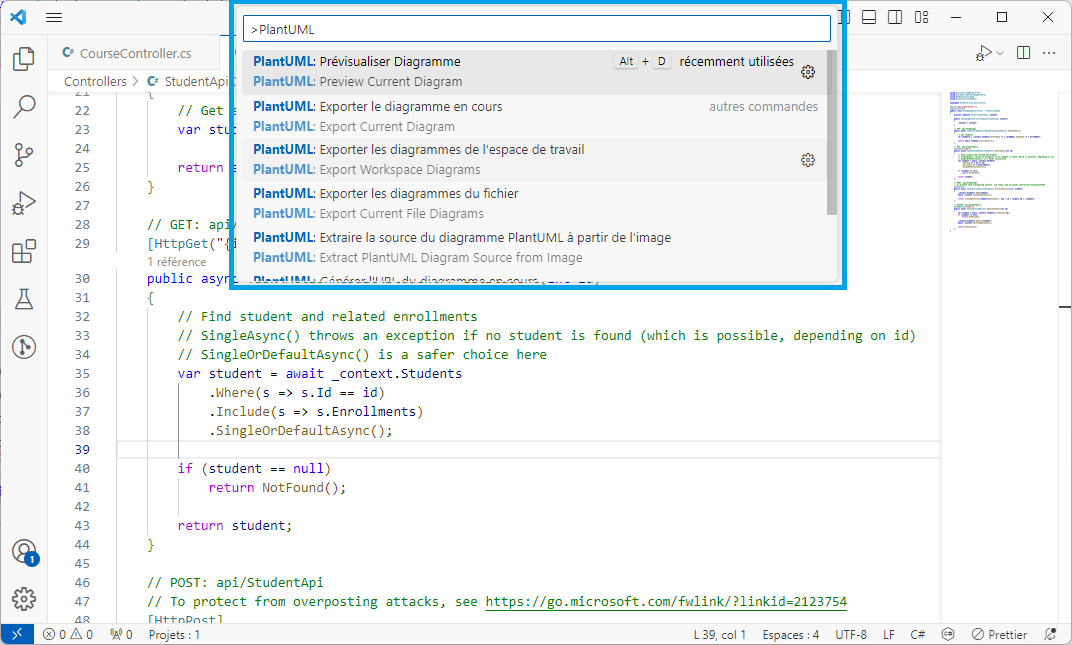
\includegraphics[height=0.4\linewidth]{figures/environnement/commande-ultime}
\end{frame}


\subsection{Le débogage}
\label{subsec:debogage}

% debug, stacktrace,

\subsection{Gestion de version}
\label{subsec:cvs}

\begin{frame}
    \frametitle{Git}

    \emph{A silly, incompetent, stupid or annoying person (usually a man).}

    \textbf{Torvalds} sarcastically quipped about the name git:
    \enquote{I'm an egotistical bastard, and I name all my projects after myself. First 'Linux', now 'git'.}

    \enquote{git} can mean anything, depending on your mood.
    \begin{itemize}
        \item Random three-letter combination that is pronounceable, and not actually used by any common UNIX command ;
        \item \enquote{Global information tracker} ;
        \item \enquote{Goddamn idiotic truckload of sh*t} ;
    \end{itemize}

    The source code for Git refers to the program as \enquote{the information manager from hell}.
\end{frame}

% Git avancé (branche rebase),
% Comment travailler

%git config --global user.name "Your Name"
%git config --global user.email "youremail@yourdomain.com"

    \section{Les pratiques du développeur}
\label{sec:pratiques}

% Réutilisation, Encapsulation maximale, Couplage faible, Cohésion forte, DRY, KISS, YAGNI
% Loi de demeter
% SOLID
% Commentaire, formattage, langue, nommage

\lstset{basicstyle=\ttfamily\tiny}

\begin{frame}
    \frametitle{SOLID}

    \begin{columns}
        \begin{column}{0.5\textwidth}
            \begin{itemize}
                \item Principe de responsabilité unique
                \item Principe ouvert/fermé
                \item Principe de substitution de Liskov
                \item Principe de ségrégation des interfaces
                \item Principe d'inversion des dépendances
            \end{itemize}
        \end{column}
        \begin{column}{0.5\textwidth}
            \begin{itemize}
                \item Single Responsibility Principle
                \item Open/closed principle
                \item Liskov substitution principle
                \item Interface segregation principle
                \item Dependency inversion principle
            \end{itemize}
        \end{column}
    \end{columns}
\end{frame}

\begin{frame}
    \frametitle{Principe de responsabilité unique}

    \begin{columns}
        \begin{column}{0.5\textwidth}
            \lstinputlisting[
                language={[Sharp]C},
                label=lst:srp-ko]
            {figures/pratiques/srp-ko.cs}
        \end{column}
        \pause
        \begin{column}{0.5\textwidth}
            \lstinputlisting[
                language={[Sharp]C},
                label=lst:srp-ok]
            {figures/pratiques/srp-ok.cs}
        \end{column}
    \end{columns}
\end{frame}

\begin{frame}
    \frametitle{Principe de responsabilité unique}

    Une classe doit avoir une et une seule raison de changer !

    \begin{itemize}
        \item La classe est plus facile à comprendre ;
        \item La classe est plus facile à maintenir ;
        \item La classe est plus réutilisable.
    \end{itemize}

    \bigskip
    Le SRP équivaut à peu près à avoir une \textbf{« cohésion élevée »}.
    On dit qu’une classe a une forte cohésion si ses comportements sont fortement liés et fortement concentrés.
    Le SRP stipule qu’une classe doit être cohérente au point d’avoir une seule responsabilité,
    où une responsabilité est définie comme \textbf{« une raison de changement »}.

\end{frame}

\begin{frame}
    \frametitle{Principe ouvert/fermé}

    \begin{columns}
        \begin{column}{0.5\textwidth}
            \lstinputlisting[
                language={[Sharp]C},
                label=lst:ocp-ko]
            {figures/pratiques/ocp-ko.cs}
        \end{column}
        \pause
        \begin{column}{0.5\textwidth}
            \lstinputlisting[
                language={[Sharp]C},
                label=lst:ocp-ok]
            {figures/pratiques/ocp-ok.cs}
        \end{column}
    \end{columns}
\end{frame}


\begin{frame}
    \frametitle{Principe ouvert/fermé}

    Vous devriez pouvoir étendre le comportement d'une classe, sans le modifier.\\
    Une classe doit être ouverte à l’extension, mais fermée à la modification.

    \begin{itemize}
        \item La classe devient robuste, flexible et réutilisable ;
        \item Moins de modification implique moins de bogue.
    \end{itemize}

\end{frame}

\begin{frame}
    \frametitle{Principe de substitution de Liskov}

    \begin{columns}
        \begin{column}{0.5\textwidth}
            \lstinputlisting[
                language={[Sharp]C},
                label=lst:lsp-ko]
            {figures/pratiques/lsp-ko.cs}
        \end{column}
        \pause
        \begin{column}{0.5\textwidth}
            \lstinputlisting[
                language={[Sharp]C},
                label=lst:lsp-ok]
            {figures/pratiques/lsp-ok.cs}
        \end{column}
    \end{columns}
\end{frame}

\begin{frame}
    \frametitle{Principe de substitution de Liskov}

    Les fonctions qui utilisent une classe de base doivent
    pouvoir utiliser des objets de classes dérivées sans le savoir.

    Lorsque les sous-classes n'adhèrent pas correctement à l'interface de la classe de base,
    il faut parcourir le code existant et tenir compte des cas particuliers impliquant les sous-classes délinquantes.
    Il s’agit d’une violation flagrante du principe ouvert/fermé.

    \bigskip
    Lors de l’apprentissage de la programmation orientée objet,
    l’héritage est généralement décrit comme une relation « est un »,
    mais elle entraîne \textbf{parfois une mauvaise utilisation de l'héritage}.

\end{frame}

\begin{frame}
    \frametitle{Principe de ségrégation des interfaces}

    \begin{columns}
        \begin{column}{0.5\textwidth}
            \lstinputlisting[
                language={[Sharp]C},
                label=lst:isp-ko]
            {figures/pratiques/isp-ko.cs}
        \end{column}
        \pause
        \begin{column}{0.5\textwidth}
            \lstinputlisting[
                language={[Sharp]C},
                label=lst:isp-ok]
            {figures/pratiques/isp-ok.cs}
        \end{column}
    \end{columns}
\end{frame}

\begin{frame}
    \frametitle{Principe de ségrégation des interfaces}

    Les clients ne devraient pas être obligés de dépendre d’interfaces qu’ils n’utilisent pas.

    Ce principe permet d'éviter le couplage involontaire entre classes.
\end{frame}

\begin{frame}
    \frametitle{ISP, OCP, and DIP… OMG WTF BBQ?}

    L'exemple précédent ne viole pas simplement la ségrégation des interfaces (ISP),
    il viole également inversion de dépendance (DIP) et le principe d'ouverture/fermeture (OCP).
    C’est assez courant, donc si vous adhérez correctement au DIP et à l’OCP,
    vous ne rencontrerez pas de nombreuses violations de l'ISP.
    Cela dit, c'est un autre moyen pratique d'évaluer la conception de votre classe.

    \bigskip
    \textbf{``Ai-je besoin de toutes les méthodes de cette interface que j'utilise ?''}

    Si la réponse est non, vous souhaiterez peut-être utiliser une interface différente
    et appliquer certains des autres principes SOLID.
\end{frame}

\begin{frame}
    \frametitle{Principe d'inversion des dépendances}

    \begin{columns}
        \begin{column}{0.5\textwidth}
            \lstinputlisting[
                language={[Sharp]C},
                label=lst:dip-ko]
            {figures/pratiques/dip-ko.cs}
        \end{column}
        \pause
        \begin{column}{0.5\textwidth}
            \lstinputlisting[
                language={[Sharp]C},
                label=lst:dip-ok]
            {figures/pratiques/dip-ok.cs}
        \end{column}
    \end{columns}
\end{frame}

\begin{frame}
    \frametitle{Principe d'inversion des dépendances}

    Les modules de haut niveau ne doivent pas dépendre de modules de bas niveau.
    Les deux devraient dépendre d’abstractions.

    Ce principe permet de réduire le couplage entre composants.

    \bigskip
    Le principe d'inversion de dépendance est essentiellement un moyen d'ajouter des fiches et des prises à votre code.
    Il vous permet de créer des modules de haut niveau indépendants des modules de bas niveau.
    Les modules de bas niveau peuvent être créés ultérieurement et sont facilement remplaçables.
\end{frame}

\begin{frame}
    \frametitle{SOLID}

    \centering
    
\includegraphics[height=100px]{figures/pratiques/srp}
    
\includegraphics[height=100px]{figures/pratiques/ocp}
    
\includegraphics[height=100px]{figures/pratiques/lsp}

    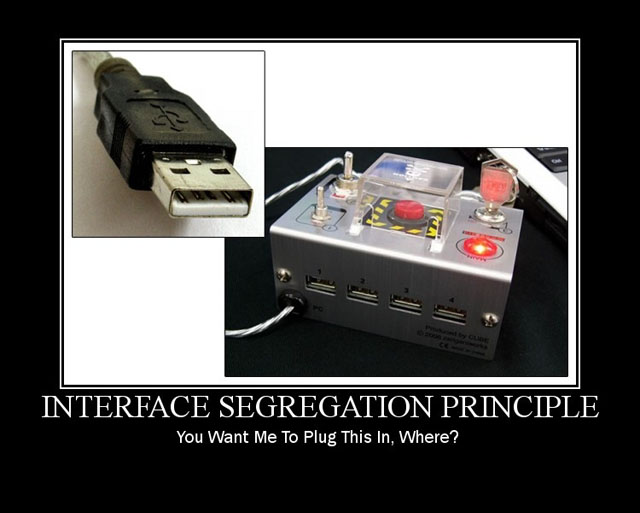
\includegraphics[height=100px]{figures/pratiques/isp}
    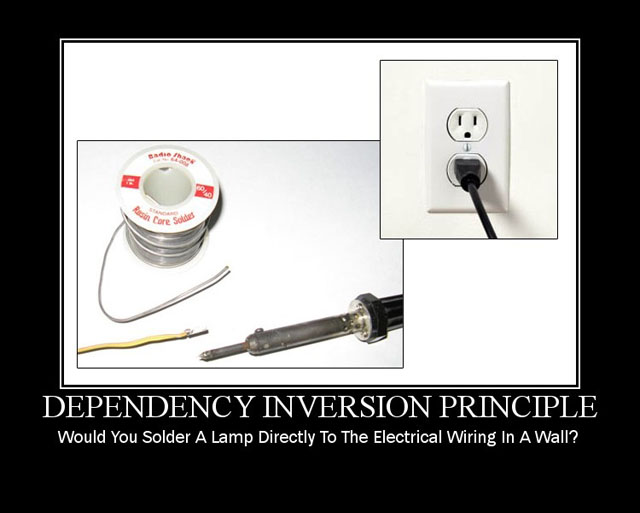
\includegraphics[height=100px]{figures/pratiques/dip}

\end{frame}

\begin{frame}
    \centering
    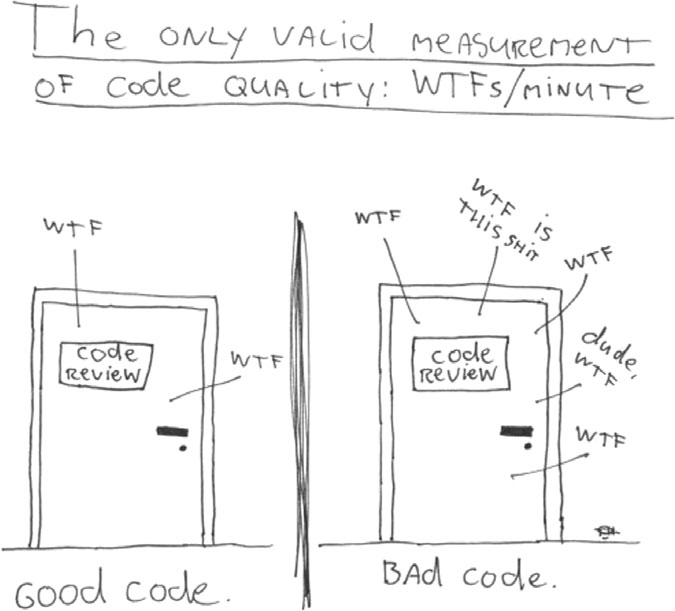
\includegraphics[height=0.5\linewidth]{figures/pratiques/wtf}
\end{frame}

    \section{Les base de données}
\label{sec:persistence}

\begin{frame}
    \frametitle{Vocabulaire}
    % DBMS, DB, Schéma
    % https://pages.cs.wisc.edu/~dbbook/openAccess/firstEdition/slides/pdfslides/mod1l1.pdf
    % https://en.wikipedia.org/wiki/Database
\end{frame}

\begin{frame}
    \frametitle{Requêtage avancée}
    % https://sql.sh/cours
\end{frame}

\begin{frame}
    \frametitle{Plan d'exécution d'une requête}
    % https://www.postgresql.org/docs/current/sql-explain.html
\end{frame}

\begin{frame}
    \frametitle{Les clés et les index}
    % https://learn.microsoft.com/fr-fr/sql/relational-databases/indexes/create-unique-indexes?view=sql-server-ver16
    % https://sql.sh/cours/index
\end{frame}

\begin{frame}
    \frametitle{Type de base de données}
    % http://igm.univ-mlv.fr/~dr/XPOSE2011/BDD/typesBD.html
    % https://en.wikipedia.org/wiki/Category:Types_of_databases
    % https://www.matillion.com/blog/the-types-of-databases-with-examples
    % https://www.mongodb.com/databases/types
    % https://duckduckgo.com/?t=ffab&q=database+type&ia=web
\end{frame}

\begin{frame}
    \frametitle{Transaction}
    % https://fr.wikipedia.org/wiki/Transaction_informatique
    % https://www.base-de-donnees.com/transaction/
\end{frame}

\begin{frame}
    \frametitle{Propriétés ACID}
    % http://igm.univ-mlv.fr/~dr/XPOSE2011/BDD/acid.html
    % https://fr.wikipedia.org/wiki/Propri%C3%A9t%C3%A9s_ACID
    % https://www.cl.cam.ac.uk/teaching//1213/Databases/db2013_L11_L12.pdf
    % https://duckduckgo.com/?t=ffab&q=database+ACID&ia=web
    % https://datascientest.com/acid
    % https://www.lebigdata.fr/acid-base-de-donnees-definition
\end{frame}

\begin{frame}
    \frametitle{Théorème CAP}
    % https://en.wikipedia.org/wiki/Eventual_consistency
    % https://fr.wikipedia.org/wiki/Th%C3%A9or%C3%A8me_CAP
    % https://www.cl.cam.ac.uk/teaching//1213/Databases/db2013_L11_L12.pdf
\end{frame}

\begin{frame}
    \frametitle{MongoDB}
    % https://www.mongodb.com/docs/manual/tutorial/query-arrays/
\end{frame}

\begin{frame}
    \frametitle{Elastic}
\end{frame}

\begin{frame}
    \frametitle{Neo4j}
    % https://neo4j.com/product/neo4j-graph-database/
\end{frame}

\begin{frame}
    \frametitle{Merise}
    % https://ineumann.developpez.com/tutoriels/merise/initiation-merise/
\end{frame}

\begin{frame}
    \frametitle{OLAP}
    % https://fr.wikipedia.org/wiki/Traitement_analytique_en_ligne#Relational_OLAP_(ROLAP)
    % https://www.lebigdata.fr/olap-online-analytical-processing
    % https://duckduckgo.com/?t=ffab&q=olap+relationnal&ia=web
\end{frame}

\begin{frame}
    \frametitle{Object–Relational Mapping (ORM)}
    % https://en.wikipedia.org/wiki/Object%E2%80%93relational_mapping#Comparison_with_traditional_data_access_techniques
    % https://www.base-de-donnees.com/orm/
\end{frame}

\begin{frame}
    \frametitle{Object–relational impedance mismatch}
    % https://en.wikipedia.org/wiki/Object%E2%80%93relational_impedance_mismatch
\end{frame}

\begin{frame}
    \frametitle{Data Access Layer (DAL)}
    %https://medium.com/swlh/designing-a-data-access-layer-part-1-f10068408e60
\end{frame}

\begin{frame}
    \frametitle{DAO}
    % https://stackoverflow.com/questions/5677518/active-record-pattern-repository-pattern-and-testability-in-java
    % https://www.baeldung.com/java-dao-pattern
    % https://www.baeldung.com/java-dao-vs-repository
    % https://medium.com/towards-polyglot-architecture/design-patterns-for-the-database-layer-7b741b126036
\end{frame}

\begin{frame}
    \frametitle{Repository}
    % https://stackoverflow.com/questions/5677518/active-record-pattern-repository-pattern-and-testability-in-java
    % https://www.baeldung.com/java-dao-pattern
    % https://www.baeldung.com/java-dao-vs-repository
    % https://medium.com/towards-polyglot-architecture/design-patterns-for-the-database-layer-7b741b126036
    % https://hashnode.com/post/which-design-pattern-do-you-prefer-active-record-or-repository-cilozoaa5016o6t53mhsdu6nu
    % https://stackoverflow.com/questions/6522009/active-records-vs-repository-pros-and-cons
\end{frame}

\begin{frame}
    \frametitle{Active Record}
    % https://medium.com/towards-polyglot-architecture/design-patterns-for-the-database-layer-7b741b126036
    % https://hashnode.com/post/which-design-pattern-do-you-prefer-active-record-or-repository-cilozoaa5016o6t53mhsdu6nu
    % https://stackoverflow.com/questions/6522009/active-records-vs-repository-pros-and-cons
    % https://en.wikipedia.org/wiki/Active_record_pattern
\end{frame}

\begin{frame}
    \frametitle{Table Module et Domain Model}
    % https://medium.com/towards-polyglot-architecture/design-patterns-for-the-database-layer-7b741b126036
\end{frame}
    \section{La collaboration dans une équipe}
\label{sec:collaboration}

%  BDD, Principe agile, XP, SCRUM, cycle de vie, exigences et tests (tdd?)

    \section{Les tests composants}
\label{sec:tests}

% unitaire, mock, méthode avancée, tester une bdd, tdd

    \section{La contenerisation}
\label{sec:contenerisation}

% Docker
% Déploiment en continue

    \section{Les patrons logiciels}
\label{sec:patrons}

    \section{Le Document d'Architecture Technique}
\label{sec:documentation}

% doc archi technique, c4

\end{document}
